\chapter{Design/Architecture \tmp{?}}

\section{Reqirements}

\tmp{TODO}

\begin{enumerate}
    \item Accurately time interrupts relative to other instructions
    \item Return RVFI to compare with the core
    \item Input interrupts and debug independently of RVFI from the core
    \item Support all same extensions the core  \textbf{\Cref{req:custom}}
    \item Modifyable to support different cores \textbf{\Cref{req:csr}}
    \item Optional: Support formal verification
    
\end{enumerate}




\section{Architecture}


\Cref{fig:architecture} shows a block diagram of the proposed architecture for the reference model and relevant surrounding modules.\tmp{explain figure}

\tmp{pipeline shell responsible for timing, ISS responsible for functional execution...}

\tmp{How is core specific funtionality is kept separate}

\begin{figure}[hbt]
    \centering
    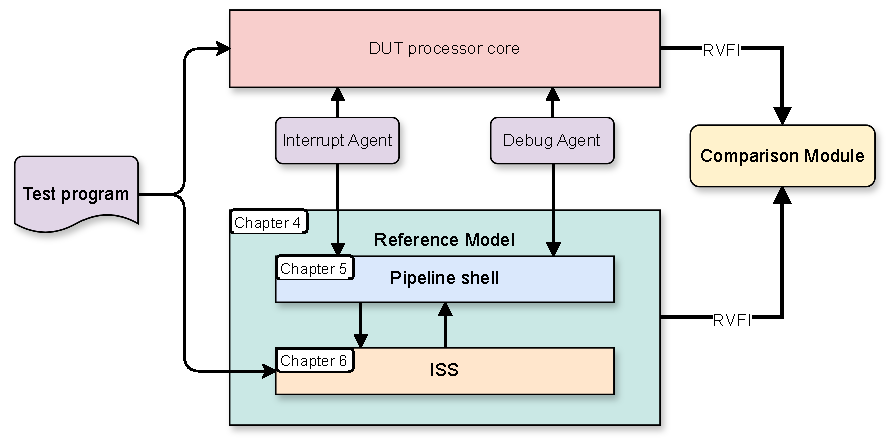
\includegraphics[width=0.75\linewidth]{figures/Architecture.pdf}
    \caption{Block diagram of the reference model architecture.}
    \label{fig:architecture}
\end{figure}


\section{Formal Verification}

Formal verification has many benefits compared to simulation as discussed in \ref{}.

A reference model that is compatible with formal methods can also be compatible with simulation tools\cite{}, so if the reference model can be built to support both formal verification and simulation it would be a very powerful tool.

Sequential \acrfull{fev} is a formal method comparing two RTL models over time. This has the possibility of working with a reference model, but this imposes several design limitations that will be discussed below.

A simpler approach without using \acrfull{fev} is to use assertions to compare the core and reference model. If the compare module used to compare the core and reference model during simulation use assertions, these can also be used for formal verification.

\subsection{Synthesisable RTL}

The currently available tools for Sequential \acrshort{fev} require that both the IMPL and SPEC models should be synthesizable \acrshort{rtl} blocks \cite{seligmanFormalVerificationEssential2015}. This limitation poses the biggest difference when compared to traditional simulation testbenches, since this means that it is not possible to use DPI functions \cite{} in order to integrate ISSs written in C/C++. This drastically limits the amount of available ISSs since most are written in C++ or other languages. 

\subsubsection{Sail}

Sail-riscv has the potential to be the model used for equivalence checking.
To achieve this the sail model must be converted to RTL code compatible with formal methods.

Sail allows the sail model to be converted to a C emulator, and multiple theorem proving tools like Coq, Isabelle/HOL, and definitions for RMEM and isla-axiomatic concurrency tools, which both focus on evaluating the relaxed-memory behavior of the \acrshort{isa}. 


Sail recently added support for compiling the model to SystemVerilog code. This could be used to model the reference model around, but at the time of writing, this feature is experimental and not mature enough to compile the sail-riscv model\footnote{\url{https://github.com/rems-project/sail/issues/420}}.

From \footnote{\url{https://github.com/rems-project/sail/releases/tag/0.17}}

\begin{quote}
    
Sail can now produce SystemVerilog output using the -sv flag. Note
that this is not intended to be human readable or produce a
synthesizable design, but is instead intended to be used with
SystemVerilog verification tools like JasperGold.
\end{quote}

The sail-riscv model can not currently be converted to SystemVerilog, as the feature is under development and not mature enough to convert the sail-riscv model at the time of writing.\cite{}
Although the sail-riscv model can not currently be converted to SystemVerilog, the rest of the reference model can still be built to support formal methods and allow us to replace the ISS with sail-riscv in the future.

One possibility is to build the rest of the reference model to support formal methods. By making the interface between the reference model and \acrshort{iss} generic, it could be possible to replace the \acrshort{iss} with SystemVerilog code generated from sail-riscv if this is possible in the future.


To verify that the rest of the reference model is compatible with formal methods, the ISS can be replaced by a "dummy" ISS while verifying the reference model with formal methods. 


We would then have two environments; a UVM simulation environment that verifies the correctness of the reference model using a C++ \acrshort{iss}, and a formal verification environment that does not test the functionality of the reference model, but checks that the reference model can run in a formal verification environment when using an RTL simulator.

If both these tests pass, future work should be to replace the dummy ISS in the formal environment with sail-riscv when the SystemVerilog generator is fully supported and verify that this works. 


\section{Reference Model language}
\tmp{TODO:}

\textbf{C++ or Systemverilog?}

-> Systemverilog in order to possibly support formal verification.
Also easier to support a pipeline etc.


\section{Testbench and comparison module architecture}

The current implementation of core-v-verif uses ImperasDV as a reference model. ImperasDV is a Verification IP, and also handles the comparison between the \acrshort{dut} and reference model \cite{imperassoftwareltdRISCVProcessorOVP2023}. In order to replace ImperasDV with the reference model, we must also implement a comparison module to compare the core with the reference model. This section will cover the integration of the reference model into the larger \gls{core-v-verif} testbench and the design of the comparison module used to compare the core and reference module.

\subsection{Compare at retirement or clock}

\tmp{Why compare at only on retirements, and not every clock?}



\subsection{Different clocks for core and reference model}

If the reference model is driven by retirements from the core, this has some implications on the timing between them.

The reference module requires the \sv{rvfi_valid} signal from the core to determine when to step the reference model.

To verify the correctness between the core and the \acrshort{rm}, we have two options regarding the clock input. We can either pass the same clock signal into the core and the \acrshort{rm}, or use an offset clock for the \acrshort{rm}.

If we pass the same clock into both, the valid signal out of the core will be one cycle delayed into the reference model as shown in \Cref{fig:1clocktiming}. When comparing the two, we have to delay the core RVFI signals so they arrive at the compare module at the same time, or use \sv{\$past()} to compare the RM with the previous cycle of the core.

\begin{figure}[hbt]
    \centering
    \begin{tikztimingtable}
      \sv{clk}    & G   6{4C} G \\ % ends with edge
      \sv{rvfi_core.valid}  & 4L 8H 12L \\
      \sv{rvfi_core}        & 4U 8D{N} 12U \\
      \sv{rvfi_rm.valid}    & 2H 10L 8H 4L \\
      \sv{rvfi_rm}          & 2D{N-1} 10U 8D{N} 4U \\
    \end{tikztimingtable}
    \caption{Timing diagram showing the \sv{rvfi_valid} signals of the core and reference model when the reference model is dependent on retirements from the core.}
    \label{fig:1clocktiming}
\end{figure}

Another solution is to use two separate clocks for the core and reference model. By having the clock of the reference model slightly offset behind the clock of the core, we get the timing diagram shown in \Cref{fig:2clocktiming} with the two clocks \sv{rvfi_core.clk} and \sv{rvfi_rm.clk} for the core and reference model, the two valid signals \sv{rvfi_core.valid} and \sv{rvfi_rm.valid}, and the rest of the rvfi signals. Here we see that the signals are equal for most of the time, and by comparing at the right clock edge, we can directly compare the equality of the signals. The lines in \Cref{fig:2clocktiming} show different clock edges we can use to compare the signals.


\tmp{How does this work with formal verification?}

using the \lstinline{set_clock_spec} with \lstinline{--pulse_offset time}  in onespin we can add multiple clocks.

\tmp{TODO: test dette}



\par\bigskip
% Vurder å bruke wavedrom
%{signal: [
%  {name: 'core.clk', wave: 'p....', period: 2},
%  {name: 'rm.clk', wave: 'P...', period:2, phase: -0.5},
%  {name: 'core.valid', wave: '0.10.', period: 2},
%  {name: 'rm.valid', wave: '0.10.', period: 2, phase: -0.5},
%], head:{
%   text:'WaveDrom example',
%   tick:0,
%   every:2,
%  	
%   }
%  }
\begin{figure}[hbt]
    \centering
    \begin{tikztimingtable}
      \sv{rvfi_core.clk}      & [C] 5{4C} C \\ % starts with edge
      \sv{rvfi_rm.clk}      & LL   5{4C} G \\ % ends with edge
      \sv{rvfi_core.valid}  & G 8L 8H 8L \\
      \sv{rvfi_core}  & G 8U 8D{N} 8U \\
      \sv{rvfi_rm.valid}    & 2H 8L 8H 6L \\
      \sv{rvfi_rm}    & 2D{N-1} 8U 8D{N} 6U \\
    \extracode
        \vertlines[red]{10}
        \vertlines[green]{14}
        \vertlines[blue]{16}
    %\extracode
    %  \tablerules
    %  \begin{pgfonlayer}{background}
    %    \foreach \n in {1,...,8}
    %      \draw [help lines] (A\n) -- (B\n);
    %  \end{pgfonlayer}
    \end{tikztimingtable}
    \caption{Timing diagram with a seperate offset clock for the reference model and the valid signals for the core and reference model.}
    \label{fig:2clocktiming}
\end{figure}

Concurrent assertions use sampled values from the beginning of the simulation step \cite[Section~4.4.3]{cernySVAPowerAssertions2015}. From \Cref{fig:2clocktiming} we see that if we sampled at the rising edge of \sv{rvfi_rm.clk} shown in red, we would sample the old value of \sv{rvfi_rm.valid} and the signals would not be equal. To fix this we can sample at a point where both signals are equal at the beginning of the simulation step, which is the case for the falling edge of \sv{rvfi_rm.clk}, the falling edge of \sv{rvfi_core.clk} or the rising edge of \sv{rvfi_core.clk}. 

If we choose the rising edge of \sv{rvfi_core.clk} we check the correctness using a \acrshort{sva} shown in \Cref{lst:pc_assertion}. To only compare the core and \acrshort{rm} at retirements, we check if \sv{rvfi_rm.valid} is high in the antecedent, before comparing the \sv{pc_rdata} signals in the consequent. This structure can then be applied to all the \acrshort{rvfi} signals.

\begin{systemverilog}[caption={Assertion comparing the PC of the \acrshort{rm}.}, label={lst:pc_assertion}]
rvfi_pc_a: assert property( @(posedge rvfi_core.clk)
    rvfi_rm.valid |-> (rvfi_rm.pc_rdata == rvfi_core.pc_rdata));
\end{systemverilog}

\subsection{Reference Model Interface}

\tmp{Rewrite:}

\begin{itemize}
    \item Should be triggered at every clock cycle, but only output on retirements?
    \item Take in interrupts and debug requests
    \item Load the ELF binary file
\end{itemize}

\textbf{\Cref{req:binaries}}

Interface requirements:

\begin{itemize}
    \item IN: clk
    \item IN: interrupt
    \item IN: debug
    \item IN: core retirement
    \item OUT: output RVFI
\end{itemize}


\subsection{ISS Interface}

\tmp{Rewrite:}

\begin{itemize}
    \item Use a wrapper to easily change out ISS later
    \item Use functions to interface with the ISS, since these work both with C functions over DPI and RTL code. Functions are not allowed to take time. This allows us to add the time ourselves with the pipeline shell.
\end{itemize}

ISS interface requirement:

\begin{itemize}
    \item Load ELF binary file \textbf{\Cref{req:binaries}}
    \item Step through one instruction and return state changes (RVFI)
    \item Inform of interrupts
    
\end{itemize}



